%%%% hw3-reqdoc.team3.tex
%%%% Requirements Documentation for sQuire
%%%% Due on BBLearn before class on Tuesday 2/9/2016

\documentclass[11pt]{report}

\usepackage{graphicx}
%\graphicspath{ {images/} }

\marginparwidth 0.5in 
\oddsidemargin 0.25in 
\evensidemargin 0.25in 
\marginparsep 0.25in
\topmargin 0.0in 
\textwidth 6in \textheight 8.5in

\title{sQuire: A Collaborative Software Development Tool}
\author{jank6275, mora5651, boss2849, bolt1003, gall7417, brec9824, snev7821, mars2681}

\begin{document}

\maketitle

\tableofcontents

\chapter{Introduction}

\section{Program Premise}
    \begin{figure}[h!]
        \caption{Squire will be a web-based collaborative software development environment with a project development center. Squire will allow multiple users to edit files and communicate in real time. Projects can be stubbed out by a user and then other users can join and/or vote to support for their favorite projects. After a certain amount of support, planning, and documentation is reached for a project, the project becomes a fully fleged ``backed'' project and then community development can start. Think ``kickstarter for code'' where people pledge their help with the project and not just money.}
        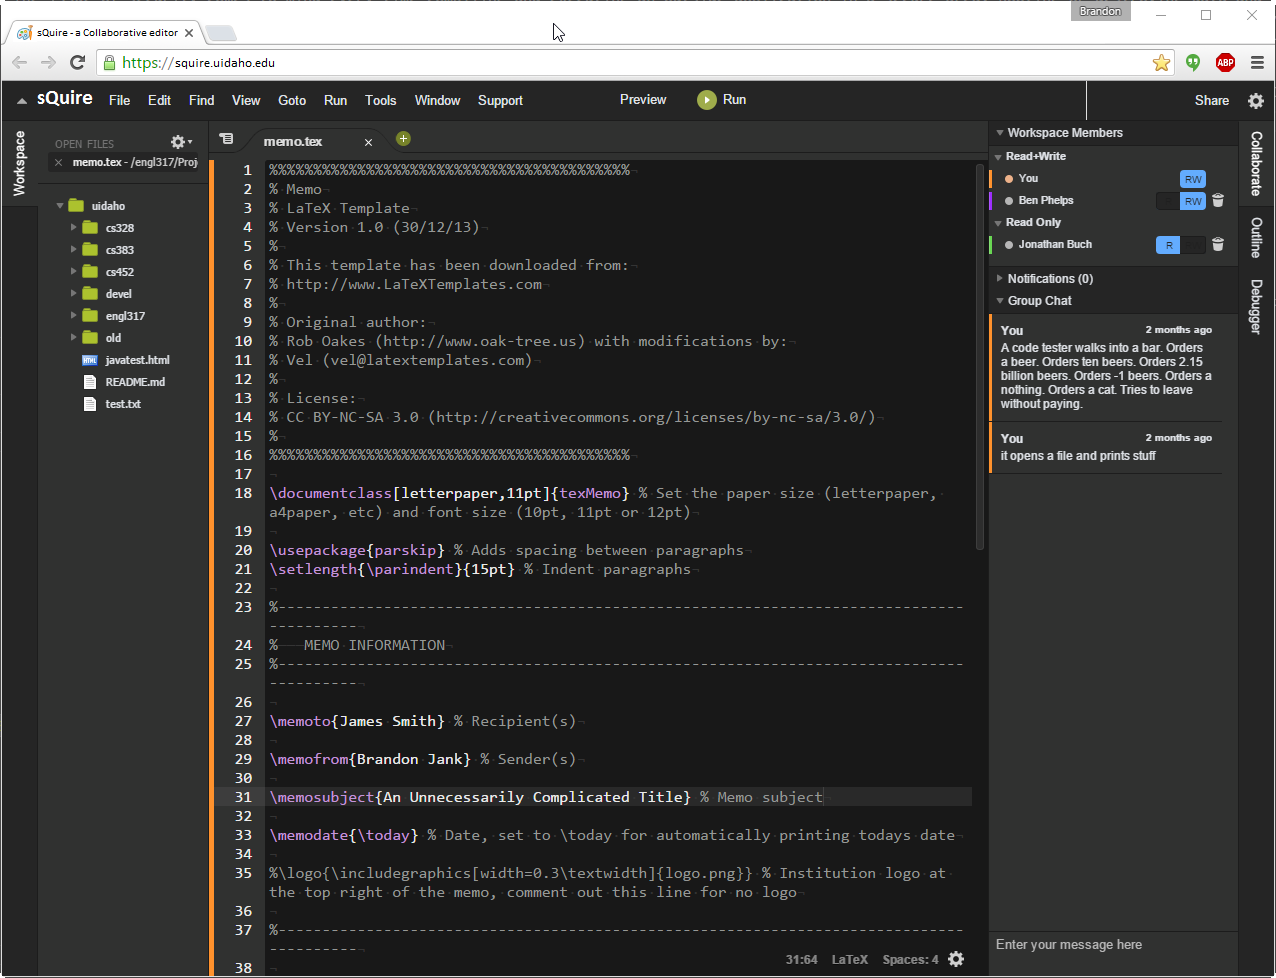
\includegraphics[width=\textwidth]{squire}
    \end{figure}

\chapter{Requirements Documentation}
    Non-functional requirements describe how the system works, while functional requirements describe what the system should do. Dr. J\'s list of requirements:
    \begin{itemize}
        \item User profiles should include persistent data including project ownerships and  memberships, friends, e-mail, profile image.
        \item Users should have easy access (background?) awareness information of other users, especially friends and members of shared projects.
        \item Resource defense strategy that includes not subjecting any sQuire server to becoming unresponsive due to a runaway program, and not allowing any sQuire server to give up shell access via an executing program in sQuire.
        \item Indication of who coded what could be background color, underline color, sidebar color, shade/fill pattern, or icon/avatar. 
        \item Since multiple people might edit a given line over its history, support for past history or anyhow multiple persons in this indication is strongly recommended.
        \item Teams should decide whether write access to shared editing should be turn-based or simultaneous
        \item Teams should decide if voice or video is essential. Voice, if supported, might be restricted as to number of listeners and/or number of simultaneous transmitters. Video, if supported, might be restricted as to number of viewers and/or number of simultaneous
        \item Capable of supporting editing, compilation, and execution of Java programs. Programs to be composed as projects and support multiple source code files across multiple directories within a shared top-level directory.
        \item Ability to import/export AND/OR function on projects/source code stored in the ordinary local file system.
        \item Multiuser, up to 32 users can share an IDE session.
        \item Syntax coloring; visual indication to see who coded what.
        \item Shared sessions should allow people to move around their view (read-only, at least) independently, and to quickly jump to where other users are looking.
        \item Users can text chat to individuals, transient shared session members, persistent project member lists, and all logged in users.
    \end{itemize}

\section{Functional Requirements}
    Functional requirements will specify a behaviour or function, for example ``Display the name, total size, available space and format of a flash drive connected to the USB port'' Other examples are ``add customer'' and ``print invoice''. Some of the more typical functional requirements include:
    \begin{itemize}
        \item Business Rules
        \item Transaction corrections, adjustments and cancellations
        \item Administrative functions
        \item Authentication
        \item Authorization levels
        \item Audit Tracking
        \item External Interfaces
        \item Certification Requirements
        \item Reporting Requirements
        \item Historical Data
        \item Legal or Regulatory Requirements
    \end{itemize}

\section{Non-Functional Requirements}
    Non-functional requirements cover all the remaining requirements which are not covered by the functional requirements. They specify criteria that judge the operation of a system, rather than specific behaviours, for example: ``Modified data in a database should be updated for all users accessing it within 2 seconds.'' Some typical non-functional requirements are:
    \begin{itemize}
        \item Performance – for example Response Time, Throughput, Utilization, Static Volumetric
        \item Scalability
        \item Capacity
        \item Availability
        \item Reliability
        \item Recoverability
        \item Maintainability
        \item Serviceability
        \item Security
        \item Regulatory
        \item Manageability
        \item Environmental
        \item Data Integrity
        \item Usability
        \item Interoperability
    \end{itemize}

\end{document}